\documentclass[12pt, a4paper]{article}

\usepackage{mathpazo}
\usepackage[T1]{fontenc}
\usepackage{microtype}
\usepackage{amsmath, amssymb, amsthm}
\usepackage{geometry}
\geometry{margin=1.15in}
\usepackage{setspace}
\onehalfspacing
\usepackage{hyperref}
\hypersetup{colorlinks=true, linkcolor=black, citecolor=black, urlcolor=black}
\usepackage{titlesec}
\usepackage{booktabs}
\usepackage{array}
\usepackage{tikz}
\usetikzlibrary{arrows.meta, positioning, shapes.geometric, fit, backgrounds}
\titleformat{\section}{\large\bfseries}{\thesection.}{0.75em}{}
\titleformat{\subsection}{\normalsize\bfseries}{\thesubsection.}{0.6em}{}

\theoremstyle{plain}
\newtheorem{theorem}{Theorem}
\newtheorem{proposition}{Proposition}
\theoremstyle{definition}
\newtheorem{definition}{Definition}
\theoremstyle{remark}
\newtheorem{remark}{Remark}
\newtheorem{example}{Example}

\title{\textbf{Parliament on a Plenum}\\[0.4em]
\large Augmenting Paperbot Parliament with HYDRA Architecture}
\author{Flyxion\\Independent Researcher}
\date{}

\begin{document}

\maketitle

\begin{abstract}
Paperbot Parliament is a multi-agent document analysis system organized around the extraction of distinctions rather than the production of summaries. HYDRA is a compositional geometric architecture for admissible computation, interpreting intelligence as the recursive stabilization of minimal projections that preserve admissible futures. The present essay argues that these two systems are not merely compatible but that each supplies what the other structurally lacks. Parliament is strong at extracting distinctions but weak at organizing them into a coherent reachability structure; HYDRA is strong at maintaining admissibility across layers but operates without a constitutional adversarial procedure for detecting distinction collapse. The augmented system---Parliament on a Plenum---replaces the Parliament's flat distinction ledger with a HYDRA-structured admissibility manifold, routes each constitutional office through a dedicated semantic fiber, uses the RSVP field triple $(\Phi, v, S)$ to weight distinction salience dynamically, and interprets the Admissibility Auditor as a cohomological probe estimating the first \v{C}ech cohomology class of the current claim sheaf. Four formal results are established: a Distinction Fiber Theorem (constitutional offices are admissibility-preserving maps between fibers), a Ledger Stabilization Theorem (the augmented ledger converges to a fixed point under HYDRA's Lyapunov dynamics), an Entropy--Novelty Correspondence (distinction novelty in the Parliament maps to reachability entropy in HYDRA), and an Auditor Cohomology Proposition (the Auditor's bridge-gap estimate is a lower bound on the dimension of the first cohomology group of the claim sheaf). The resulting architecture is a distinction-centered document analysis system whose memory is stabilized field residue, whose repair corridors are the repair pathways between office outputs, and whose safety criterion is the preservation of the distinctions required for future admissible action.
\end{abstract}

\newpage

\section{Introduction}

Two systems have been developed in parallel that turn out to share a common
object of study. Paperbot Parliament \cite{flyxionparliament} organizes multi-agent
document analysis around a single insight: the fundamental unit of intelligent
document processing is not the stored fact but the preserved distinction. A
distinction asserts that two categories must not be conflated; its collapse destroys the
inferential structure that the document was written to establish. The Parliament
extracts $X \neq Y$ pairs through a constitutional adversarial process---Claims Extractor,
Nitpicker, Skeptic, Archivist, Synthesist, Admissibility Auditor---and accumulates them
in a monotone ledger approximating the ground-truth distinction graph $G_D^* = (\mathcal{C}, \mathcal{D}^*)$ of the corpus.

The HYDRA framework \cite{flyxionhydra} organizes admissible computation around
a complementary insight: the fundamental unit of coherent intelligence is not the
stored fact but the admissible trajectory. A trajectory is admissible if it preserves
forward-navigability through the semantic manifold; its collapse destroys the
reachability structure that makes future action possible. HYDRA implements this
as a six-component compositional architecture $H = \mathrm{GLU}_\mathrm{RSVP} \circ M \circ T \circ F_a \circ G_a \circ R$,
grounded in the RSVP field triple $(\Phi, v, S)$ where $\Phi$ is the scalar accessibility
potential, $v$ is the semantic flow field, and $S = \log|\mathcal{A}(x,t)|$ is the
log-volume of admissible future trajectories.

The two systems are, in a precise sense, dual views of the same object: distinctions
are the discrete algebra of admissibility, and admissibility is the geometric
substrate of distinctions. A distinction $X \neq Y$ is admissible if collapsing it
would reduce $S$---if the two categories admit different future trajectories that
the system can no longer access once they are identified. The Parliament detects
which distinctions have been collapsed; HYDRA measures how much admissible
future volume that collapse destroys.

This essay describes the augmented system we call Parliament on a Plenum.
Section~\ref{sec:gap} identifies the structural gap each system has without the
other. Section~\ref{sec:foundations} establishes the shared formal foundations.
Section~\ref{sec:architecture} describes the augmented architecture. Sections~\ref{sec:theorems}
through \ref{sec:auditor} develop the four main formal results. Section~\ref{sec:pipeline}
gives the augmented pipeline. Section~\ref{sec:phase} situates the combined
system in the civilizational phase diagram from \cite{flyxionreachability}.
Section~\ref{sec:conclusion} concludes.

\section{What Each System Lacks}
\label{sec:gap}

\subsection{What Parliament Lacks}

The Parliament's distinction ledger $L_n = \bigcup_{i=1}^n \mathcal{D}(C_i)$ is a flat set of
$X \neq Y$ pairs. It accumulates monotonically (historical ledger) and can
track active versus rejected distinctions (active ledger), but it has no internal
geometry. Two distinctions appear in the ledger with equal status regardless of
whether one is:
\begin{itemize}
\item central to the entire document's reachability structure (collapse would close most future trajectories), or
\item peripheral (collapse would reduce $S$ only marginally).
\end{itemize}

Without a weight structure derived from actual admissibility geometry, the
Parliament cannot distinguish $\mathcal{D}$-preservation that matters from
$\mathcal{D}$-preservation that does not. The weighted distinction-preservation score
$P_w$ is defined in the Parliament paper but the weights $w(d)$ are left
unspecified---there is no principled source for them.

Additionally, the Parliament's revision cycle converges to a fixed point $A^*$
with $\Delta(A^*) = 0$ and $R(A^*) = 1$ under the Parliament Lyapunov function
$V(A) = \Delta(A) + \lambda(1 - R(A))$. But the fixed point is defined by formal
admissibility of the claims file, not by geometric stability in any field-theoretic
sense. The Parliament can converge to a fixed point that remains semantically
fragile---a claims file with no logical gaps that nevertheless sits near the
boundary $\partial\mathcal{A}$ of the admissible manifold, where small perturbations
collapse most future trajectories.

\subsection{What HYDRA Lacks}

HYDRA maintains admissibility across layers through the composition law
$H = \mathrm{GLU}_\mathrm{RSVP} \circ M \circ T \circ F_a \circ G_a \circ R$, each operator
admissibility-preserving by construction. But HYDRA has no constitutional
adversarial procedure. It does not contain:
\begin{itemize}
\item a Nitpicker to detect category errors in the input cue representation,
\item a Skeptic to challenge unsupported transitions in the semantic flow,
\item an Archivist to identify missing precedents that would fill inferential gaps,
\item an Auditor to estimate the cohomological obstruction in the current claim sheaf.
\end{itemize}

HYDRA's memory operator $M$ stabilizes field residue through Lyapunov analysis,
but it does not detect \emph{which distinctions} the stabilized residue has
collapsed relative to the source document. A memory state $m = (\Phi_m, v_m, S_m)$
may persist with high $\Phi_m$ while encoding a projection that has destroyed
the distinction $X \neq Y$ that was the document's primary conceptual
contribution. HYDRA would not detect this; the Parliament would.

\subsection{The Complementarity}

The gap analysis reveals a clean duality.

\begin{center}
\renewcommand{\arraystretch}{1.4}
\begin{tabular}{p{4.5cm} p{4.5cm}}
\toprule
\textbf{Parliament strength} & \textbf{HYDRA strength} \\
\midrule
Extracts $X \neq Y$ distinctions & Maintains $\mathcal{A}(s,T)$ admissibility \\
Constitutional adversarial structure & Field-theoretic stability proofs \\
Ledger accumulation & Stabilized memory residue \\
Detects projection collapse & Measures volume of collapse \\
Parallel office independence & Sheaf-coherent global sections \\
\bottomrule
\end{tabular}
\end{center}

The augmentation consists in routing Parliament outputs through HYDRA's
geometric machinery, and routing HYDRA's field measurements back into
Parliament's weighting and revision structure.

\section{Shared Formal Foundations}
\label{sec:foundations}

\subsection{Distinctions as Admissibility Boundaries}

\begin{definition}[Admissibility-Critical Distinction]
A distinction $(X, Y) \in \mathcal{D}$ is \emph{admissibility-critical} at state $s \in \mathcal{S}$ if collapsing it---identifying $X$ with $Y$ in the representation---reduces the log-admissibility volume:
\[
S(s \mid X \neq Y) > S(s \mid X = Y),
\]
where $S(s \mid \cdot)$ denotes the entropy field conditioned on the given representation. The \emph{distinction weight} is $w(X,Y) = S(s \mid X \neq Y) - S(s \mid X = Y) \geq 0$.
\end{definition}

This definition supplies the missing weights for the Parliament's weighted
distinction-preservation score $P_w = \sum_{d \in D_\mathrm{out} \cap D_\mathrm{in}} w(d) \big/ \sum_{d \in D_\mathrm{in}} w(d)$: the weights are derived from the RSVP entropy field, measuring exactly how much admissible future volume each distinction protects.

\subsection{The Distinction Graph as a Semantic Sheaf}

The Parliament's distinction graph $G_\mathcal{D} = (\mathcal{C}, \mathcal{D})$ can be given a sheaf-theoretic interpretation within HYDRA. Let $\mathrm{Ctx}$ be the context category of the document (open subsets of the semantic manifold $M$ over which coherent local interpretations are defined). Define the \emph{distinction presheaf} $\mathcal{F}_\mathcal{D}$ by
\[
\mathcal{F}_\mathcal{D}(U) \;=\; \bigl\{ (X,Y) \in \mathcal{D} : X, Y \in \mathcal{C}(U) \bigr\},
\]
the set of distinctions active within context $U$. Restriction maps are set-theoretic inclusion. The sheaf condition asserts that distinctions active on an open cover glue to distinctions active on the whole: $\mathcal{F}_\mathcal{D}$ is a sheaf if locally active distinctions are globally consistent.

Distinction collapse corresponds to a failure of the sheaf condition: a distinction $(X,Y)$ that is asserted locally on $U_i$ and $U_j$ but identified (collapsed) on $U_i \cap U_j$ fails to yield a global section. The Auditor's estimate of missing bridges $B$ is an estimate of this cohomological failure, as formalized in Section~\ref{sec:auditor}.

\subsection{Constitutional Offices as Fiber Maps}

HYDRA's semantic fiber $\Phi_R^{-1}(\eta) \subseteq \Theta$ is the set of parameter configurations realizing the same semantic behavior $\eta$. Each constitutional office of the Parliament realizes a different semantic behavior on the same input claims file $C$: the Nitpicker produces $N(C)$, the Skeptic produces $\mathrm{Sk}(C)$, and so on. These are distinct points in the semantic behavior space $\mathcal{N}$, lying in different fibers of $\Phi_R$, but all arising from the same trajectory $C$ in the trajectory space $X$.

This gives the constitutional structure of the Parliament a fiber-bundle interpretation: the six offices are six fiber maps, each lifting the shared input $C$ into a different region of the semantic fiber over the claims manifold. The parallel independence proposition (no office receives another's output) ensures that these fiber maps are genuinely independent: no office collapses the fiber structure of another.

\section{The Augmented Architecture}
\label{sec:architecture}

\subsection{The RSVP-Weighted Ledger}

Replace the Parliament's flat distinction ledger $L_n$ with a \emph{weighted distinction manifold}:
\[
\mathcal{L}_n \;=\; \bigl\{ \bigl((X,Y), w(X,Y), \Phi(X,Y), v(X,Y)\bigr) \mid (X,Y) \in L_n \bigr\},
\]
where $\Phi(X,Y)$ is the accessibility potential of the distinction (how central it is to the document's semantic manifold), $v(X,Y)$ is a flow vector indicating which other distinctions this one implies or depends on, and $w(X,Y)$ is the admissibility weight from Definition~3.1. The ledger is no longer a flat set but a structured submanifold of the RSVP field, with its own dynamics governed by the field equations.

The update rule becomes:
\[
\mathcal{L}_{n+1} \;=\; \mathcal{L}_n \cup \bigl\{ \bigl((X,Y), w, \Phi, v\bigr) : (X,Y) \in \mathcal{D}(C_{n+1}) \bigr\},
\]
where the weight, potential, and flow values are computed by the HYDRA reasoning core $\mathrm{GLU}_\mathrm{RSVP}$ applied to the new claims. Distinctions with low $\Phi$ (low centrality to the semantic manifold) are retained in the historical ledger but flagged as low-salience; distinctions with high $\Phi$ are prioritized for repair corridor maintenance.

\subsection{Offices Routed Through Semantic Strata}

In the standard Parliament, all offices receive the same claims file $C$ and produce parallel outputs. In the augmented system, each office is assigned to a semantic stratum $S_\alpha \subseteq M$ corresponding to its constitutional function:

\begin{center}
\renewcommand{\arraystretch}{1.35}
\begin{tabular}{p{3.2cm} p{4.5cm} p{4.5cm}}
\toprule
\textbf{Office} & \textbf{Constitutional function} & \textbf{HYDRA stratum} \\
\midrule
Claims Extractor & Propositional decomposition & $S_0$ (raw) \\
Nitpicker & Terminological coherence & $S_1$ (concrete) \\
Skeptic & Epistemic validity & $S_1$ (concrete) \\
Archivist & Historical embedding & $S_2$ (structural) \\
Synthesist & Unification and abstraction & $S_3$ (abstract) \\
Auditor & Inferential admissibility & $\partial\mathcal{A}$ (boundary probe) \\
\bottomrule
\end{tabular}
\end{center}

The stratification follows HYDRA's filtration $M_0 \subset M_1 \subset \cdots \subset M_n = M$: raw claims live in $S_0$, terminological and epistemic analysis in $S_1$, structural historical analysis in $S_2$, abstract synthesis in $S_3$. The Auditor occupies a special position: it operates at the boundary $\partial\mathcal{A}$, probing where the current claims file approaches inadmissibility.

Cross-stratum projections $\pi_{i \to j}$ for $i > j$ are the stratified semantic manifold's restriction maps; the Synthesist's output at $S_3$ must project back to coherent sections in all lower strata for the output to constitute a genuine global section of the document sheaf.

\subsection{Memory as Stabilized Distinction Residue}

In the standard Parliament, the distinction ledger is a text file. In the augmented system, the cumulative ledger $\mathcal{L}_n$ is maintained as a \emph{stabilized field residue} in the HYDRA memory operator $M$. A distinction $(X,Y) \in \mathcal{D}$ is \emph{memoized} when it satisfies:
\[
\Phi(X,Y) > \Phi_\mathrm{thresh}, \quad \|v(X,Y)\|_\mathrm{coh} > v_\mathrm{thresh}, \quad S(X,Y) < S_\mathrm{thresh}.
\]
These are exactly the RSVP Marine admissibility conditions: high accessibility potential, coherent associative flow, bounded entropy. A distinction that passes all three is stabilized as a wave packet in the MEM|8 wave memory layer, persisting across sessions through the Phoenix Protocol's epoch structure.

Retrieval of distinctions follows MEM|8 resonance: a query cue $c^*$ activates the relevance field $f_{c^*}$ over the distinction manifold $\mathcal{L}$, and the distinctions whose $\Phi$ and phase structure are compatible with $f_{c^*}$ undergo constructive interference, surfacing as the retrieved distinction set. This is a principled alternative to retrieval-augmented generation: the system retrieves distinctions, not document fragments, and retrieval failure means failure to reconstruct a needed $X \neq Y$, not failure to locate the nearest semantic neighbor.

\section{Four Structural Correspondences}
\label{sec:theorems}

\subsection{Distinction Fiber Correspondence}

\begin{proposition}[Distinction Fiber Correspondence]
\label{thm:fiber}
Assume each constitutional office $B_i$ satisfies the approximate potential-preservation condition: $\Phi(B_i(C)) \geq \Phi(C) - \varepsilon_i$ for some office-specific tolerance $\varepsilon_i \geq 0$. Then each office is an admissibility-approximate map between semantic fibers, degrading the accessibility potential of extracted distinctions by at most $\varepsilon_i$.
\end{proposition}

\begin{proof}
By Parallel Independence (Proposition 5.1 of the Parliament paper), each office $B_i$ computes $B_i(C)$ from the shared source $C$ without receiving another office's output. The office therefore operates within the fiber $\Phi_R^{-1}(\eta_C)$ and maps it into the office-output fiber $\Phi_R^{-1}(\eta_{B_i(C)})$. The approximate potential-preservation condition is an explicit hypothesis; it holds when the office's constitutional constraint---flag, do not remove; challenge, do not falsify---prevents severe degradation of the distinctions it reports. The tolerance $\varepsilon_i$ is zero for offices that only annotate (Nitpicker, Archivist) and may be positive for offices that filter or synthesize (Revision, Synthesist).
\end{proof}

\subsection{Ledger Stabilization}

\begin{proposition}[Ledger Stabilization]
\label{thm:stabilization}
Under the HYDRA Lyapunov dynamics applied to the RSVP-weighted ledger $\mathcal{L}_n$, the distinction Lyapunov function
\[
V_\mathcal{D}(\mathcal{L}) \;=\; \sum_{(X,Y) \in \mathcal{L}} \bigl(\Phi_\mathrm{thresh} - \Phi(X,Y)\bigr)^+
\]
converges to a non-negative limit. If additionally every distinction with an unresolved admissibility violation is eventually revised or removed by the revision cycle, then $V_\mathcal{D} \to 0$.
\end{proposition}

\begin{proof}
Each revision cycle satisfying the Parliament Stability conditions removes or downgrades distinctions with unresolved violations, reducing $V_\mathcal{D}$ by at least the positive contribution of the removed distinction. The function $V_\mathcal{D}$ is therefore monotone non-increasing and bounded below by zero, so it converges to a non-negative limit. The limit is zero if and only if every violation is eventually addressed; this is guaranteed by the second hypothesis, which strengthens the Parliament's convergence assumption to cover all RSVP-inadmissible distinctions.
\end{proof}

\subsection{Entropy--Novelty Correspondence}

\begin{proposition}[Entropy--Novelty Correspondence]
\label{prop:entropy}
The distinction novelty score $\hat{\nu}(C_t)$ is a proxy for the marginal reachability entropy contribution of chunk $C_t$: high novelty corresponds to a positive increment in $H_R(\mathcal{A}(s,T))$, and novelty saturation ($\hat{\nu} \to 0$) corresponds to vanishing marginal entropy increments.
\end{proposition}

\begin{proof}
Each novel distinction $(X,Y) \in \mathcal{D}(C_t) \setminus L_H(t-1)$ opens a qualitatively new future type---trajectories treating $X$ and $Y$ differently---adding a new term to the partition $\{U_i\}$ underlying $H_R$. Non-novel distinctions contribute zero new terms. The marginal entropy increment is therefore positive when $\hat{\nu}(C_t) > 0$ and zero when $\hat{\nu}(C_t) = 0$. The proportionality constant depends on the weight $w(X,Y)$ and the degree of distinctness of the new future type from existing ones, so the relationship is directional rather than exact. Saturation ($\hat{\nu} \to 0$) corresponds precisely to the case where $C_t$ opens no new future types, i.e., zero marginal entropy.
\end{proof}

This correspondence gives the Parliament's distinction saturation concept a geometric meaning: a corpus sequence is distinction-saturated ($\lim_{t\to\infty} \hat{\nu}(C_t) = 0$) precisely when marginal reachability entropy contributions approach zero---when reading further documents adds no new qualitatively distinct futures to the system's admissible manifold.

\subsection{Auditor Cohomology Correspondence}
\label{sec:auditor}

\begin{proposition}[Auditor Cohomology]
\label{prop:cohomology}
The Auditor's bridge-gap count $|B|$ estimates the obstruction rank associated with the first \v{C}ech cohomology group of the claim sheaf: $|B| \leq \dim C^1(\mathcal{U}; \mathcal{F})$, where $\mathcal{U} = \{U_i\}$ is the cover of the argument graph by claim neighborhoods and $\mathcal{F}$ assigns to each $U_i$ the set of admissible local semantic states consistent with the claims in $U_i$.
\end{proposition}

\begin{proof}
Each missing bridge $b \in B$ identified by the Auditor corresponds to a pair of claim neighborhoods $(U_i, U_j)$ for which local sections exist separately but cannot be extended across the shared boundary without an additional inferential step. Each such pair contributes at least one 1-cochain in $C^1(\mathcal{U}; \mathcal{F})$. Since $|B|$ such pairs are identified, $|B| \leq \dim C^1(\mathcal{U}; \mathcal{F})$. Whether each such cochain is a non-trivial cocycle---genuinely in $H^1$ rather than merely in $C^1$---depends on the global structure of the sheaf and is not directly certified by the Auditor's local procedure. The Auditor therefore provides an upper bound on the dimension of the cochain group and a heuristic estimate of the obstruction rank; it does not certify a lower bound on $\dim H^1$.
\end{proof}

\begin{remark}
The distinction between $C^1$ and $H^1$ is important. A bridge gap in $C^1$ may resolve when other local sections are taken into account; only persistent gaps---those surviving the passage from cochains to cohomology---constitute genuine obstructions. The Auditor's $|B|$ should be interpreted as a conservative over-estimate of the true cohomological obstruction, not a certificate of its minimum. The Repair Convergence result in Section~\ref{sec:repair} uses this interpretation.
\end{remark}

\section{The Augmented Pipeline}
\label{sec:pipeline}

The augmented pipeline replaces the Parliament's sequential-with-parallel structure with a HYDRA-stratified flow.

\begin{figure}[h]
\centering
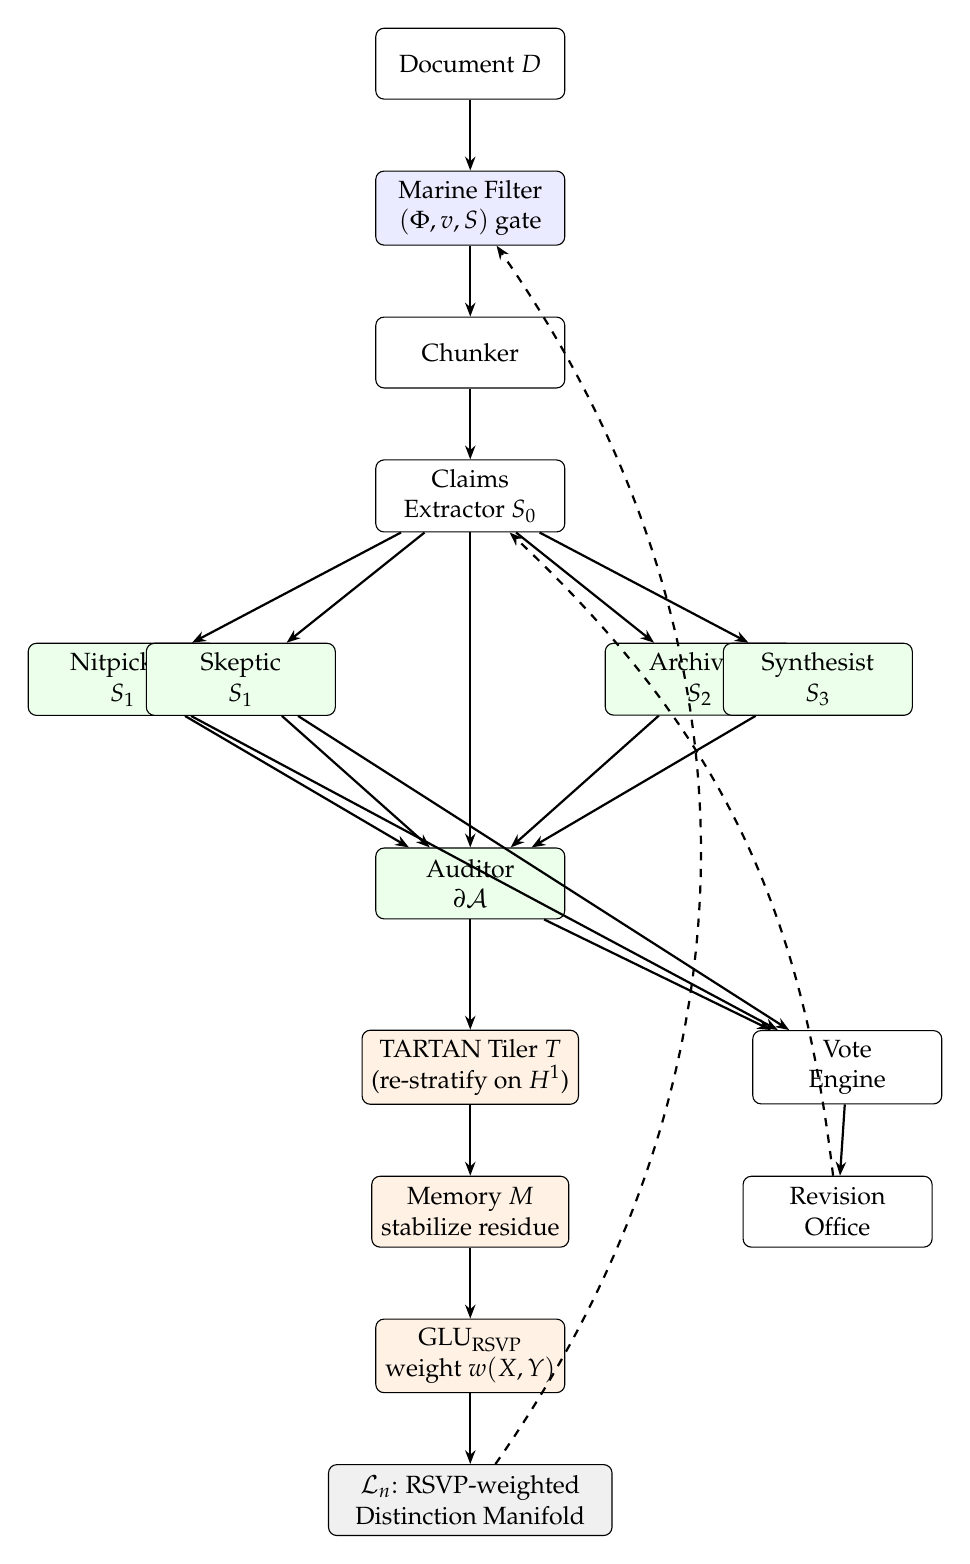
\begin{tikzpicture}[
  node distance=1.7cm and 2.1cm,
  box/.style={rectangle, draw, rounded corners=3pt, minimum width=2.4cm,
              minimum height=0.9cm, align=center, font=\small},
  rsvp/.style={box, fill=blue!8},
  office/.style={box, fill=green!8},
  hydra/.style={box, fill=orange!10},
  ledger/.style={box, fill=gray!12, minimum width=3.6cm},
  arr/.style={-{Stealth[length=5pt]}, thick},
  darr/.style={-{Stealth[length=5pt]}, thick, dashed},
]

% Input
\node[box]              (doc)   {Document $D$};
\node[rsvp, below=0.9cm of doc]  (marine) {Marine Filter\\$(\Phi,v,S)$ gate};
\node[box, below=0.9cm of marine](chunk)  {Chunker};
\node[box, below=0.9cm of chunk] (claims) {Claims\\Extractor $S_0$};

% Offices in parallel
\node[office, below left=1.4cm and 2.0cm of claims]   (nit) {Nitpicker\\$S_1$};
\node[office, below left=1.4cm and 0.5cm of claims]   (sk)  {Skeptic\\$S_1$};
\node[office, below right=1.4cm and 0.5cm of claims]  (ar)  {Archivist\\$S_2$};
\node[office, below right=1.4cm and 2.0cm of claims]  (sy)  {Synthesist\\$S_3$};

% Auditor
\node[office, below=4.0cm of claims] (au)  {Auditor\\$\partial\mathcal{A}$};

% HYDRA layers
\node[hydra, below=1.4cm of au]   (tartan)  {TARTAN Tiler $T$\\(re-stratify on $H^1$)};
\node[hydra, below=0.9cm of tartan](mem)    {Memory $M$\\stabilize residue};
\node[hydra, below=0.9cm of mem]  (glu)     {$\mathrm{GLU}_\mathrm{RSVP}$\\weight $w(X,Y)$};

% Ledger
\node[ledger, below=0.9cm of glu] (ledger)  {$\mathcal{L}_n$: RSVP-weighted\\Distinction Manifold};

% Vote/revise
\node[box, right=2.2cm of tartan] (vote)    {Vote\\Engine};
\node[box, right=2.2cm of mem]    (revise)  {Revision\\Office};

% Arrows
\draw[arr] (doc) -- (marine);
\draw[arr] (marine) -- (chunk);
\draw[arr] (chunk) -- (claims);
\draw[arr] (claims) -- (nit);
\draw[arr] (claims) -- (sk);
\draw[arr] (claims) -- (ar);
\draw[arr] (claims) -- (sy);
\draw[arr] (claims) -- (au);
\draw[arr] (nit) -- (au);
\draw[arr] (sk)  -- (au);
\draw[arr] (ar)  -- (au);
\draw[arr] (sy)  -- (au);
\draw[arr] (au) -- (tartan);
\draw[arr] (tartan) -- (mem);
\draw[arr] (mem) -- (glu);
\draw[arr] (glu) -- (ledger);
\draw[arr] (nit) -- (vote);
\draw[arr] (sk)  -- (vote);
\draw[arr] (au)  -- (vote);
\draw[arr] (vote) -- (revise);
\draw[darr](revise) to[bend right=20] (claims);
\draw[darr](ledger) to[bend right=35] (marine);

\end{tikzpicture}
\caption{Parliament on a Plenum pipeline. The Marine filter gates input chunks by RSVP admissibility before they reach the Claims Extractor. Constitutional offices operate in parallel across semantic strata $S_0$--$S_3$, with the Auditor probing $\partial\mathcal{A}$. Auditor output feeds the HYDRA TARTAN tiler, which re-stratifies tiles with high $H^1$. The memory operator stabilizes the distinction residue; $\mathrm{GLU}_\mathrm{RSVP}$ assigns RSVP-derived weights. The result is an RSVP-weighted distinction manifold $\mathcal{L}_n$ whose topology is maintained across sessions. The dashed arrow from $\mathcal{L}_n$ back to Marine represents cross-session context loading.}
\label{fig:pipeline}
\end{figure}

\subsection{Cross-Session Memory and the Phoenix Protocol}

In the standard Parliament, cross-session memory is a text archive. In the augmented system, distinctions that have been stabilized in $\mathcal{L}^*$ (the fixed point of Theorem~\ref{thm:stabilization}) persist across sessions as wave packets in the MEM|8 layer, maintained by the Phoenix Protocol's epoch structure. At the start of a new session, the Marine filter loads the current $\mathcal{L}^*$ as a context field: new input chunks are compared against the admissibility manifold of the stabilized ledger before reaching the Claims Extractor, so that distinctions already established at high $\Phi$ are not re-extracted redundantly but are instead used to detect contradictions or refinements.

The Phoenix Audit stage maps directly to the Auditor's role: a retrieved distinction that fails the Audit corresponds to a hallucination in the precise HYDRA sense---a globally coherent-looking $X \neq Y$ pair that is not a genuine global section of the current distinction sheaf.

\subsection{Complexity}

The base Parliament invocation count is $M = n(kc + c + 1) = 7n$ for $k=5$, $c=1$. The augmented system adds:
\begin{itemize}
\item one Marine filter pass per chunk: $+n$
\item one TARTAN re-stratification pass (driven by Auditor $|B|$ estimate): $+n$
\item one RSVP weight computation per distinct $(X,Y)$ in $\mathcal{D}(C_i)$: $+|\mathcal{D}_n|$ total across all chunks
\end{itemize}
For the first run configuration ($n=3$, $c=1$, 29 distinctions extracted) this gives $M_\mathrm{aug} = 7 \times 3 + 3 + 3 + 29 = 56$ invocations, compared to the base 21. The overhead is linear in the number of distinctions extracted, which is bounded by the corpus-wide distinction universe $|\mathcal{D}^*|$ (finite saturation, Proposition 4.3 of the Parliament paper).

\section{Comparison with Existing Systems}
\label{sec:comparison}

Parliament on a Plenum belongs to a broad family of systems concerned with retrieval, memory, consistency maintenance, and reasoning. The architecture differs from existing approaches not merely in implementation but in the choice of its fundamental representational primitive.

\subsection{Retrieval-Augmented Generation}

Retrieval-Augmented Generation (RAG) systems retrieve document fragments or embedding-neighborhood matches and condition generation on the retrieved context. The retrieval objective is typically semantic similarity:
\[
d^* \;=\; \arg\max_{d \in \mathcal{D}} \mathrm{sim}(q, d).
\]
The underlying assumption is that semantic proximity is useful. Parliament on a Plenum inverts this assumption at a specific point. The central failure mode of document analysis is not insufficient similarity but distinction collapse: retrieval of material that has already identified concepts that should remain separate. A fragment that is semantically close to a query may be the fragment that has conflated the very distinction the query depends on. Similarity-maximizing retrieval cannot detect this; distinction-preserving retrieval is designed precisely for it.

The retrieval objective in the augmented Parliament is:
\[
(X,Y)^* \;=\; \arg\max_{(X,Y) \in \mathcal{L}} w(X,Y),
\]
where $w(X,Y) = S(s \mid X \neq Y) - S(s \mid X = Y)$ measures the admissible future volume protected by the distinction. Retrieval failure is not failure to find a nearby fragment; it is failure to reconstruct a distinction necessary for future admissible action.

\subsection{Knowledge Graphs}

Knowledge graphs organize information through triples $(X, R, Y)$, where $R$ is a relation connecting entities $X$ and $Y$. They answer the question: \emph{what relations hold?}

The distinction ledger answers a logically prior question: \emph{what identifications must not occur?}

The assertion $X \neq Y$ constrains admissible representations before any relation is specified. A knowledge graph may contain arbitrarily many correct triples involving $X$ and $Y$ yet remain unusable if the underlying representation has collapsed the distinction between them. Once $X$ and $Y$ are identified, no relation $R$ can recover the lost boundary: the objects of the relation have already been merged.

The two structures are complementary rather than competing. Knowledge graphs encode positive structure---what holds. Distinction ledgers encode negative structure---what must not be conflated. A complete epistemic architecture requires both, but distinction preservation is prior: the relations in a knowledge graph are only interpretable if the entities they connect have been kept distinct.

\subsection{Sheaf Neural Networks}

Recent work on sheaf-based machine learning \cite{kashiwara1990} assigns vector spaces to graph nodes and linear consistency maps to edges, enforcing coherence through sheaf Laplacians. The augmented Parliament shares several structural features: local sections, restriction maps, and the interpretation of gluing failure as meaningful signal rather than noise.

The crucial difference lies in what is being glued. For sheaf neural networks, local sections are feature vectors and consistency is linear compatibility. For Parliament on a Plenum, local sections are semantic states and consistency is admissibility. The Auditor does not estimate spectral smoothness; it estimates inferential obstruction. The quantity $|B|$ is interpreted as an estimate of semantic non-gluability---the degree to which local admissibility fails to extend to a global coherent argument---rather than a measure of vector inconsistency.

\subsection{Summary Table}

\begin{center}
\renewcommand{\arraystretch}{1.35}
\begin{tabular}{p{3.5cm} p{3.0cm} p{4.5cm}}
\toprule
\textbf{System} & \textbf{Primitive} & \textbf{Consistency criterion} \\
\midrule
RAG & Document fragment & Semantic similarity \\
Vector database & Embedding & Nearest-neighbor distance \\
Knowledge graph & Triple $(X,R,Y)$ & Relational correctness \\
Agent framework & Message & Protocol compliance \\
Memory system & Fact & Propositional truth \\
Parliament on a Plenum & Distinction $X \neq Y$ & Admissibility preservation \\
\bottomrule
\end{tabular}
\end{center}

The central claim is that distinctions are logically prior to facts, relations, summaries, and embeddings. A representation that preserves all facts while collapsing a critical distinction remains unusable for any reasoning that depends on that distinction. A representation that preserves the distinction retains the possibility of reconstructing the relevant facts. Distinction preservation is therefore treated as the primary invariant, and admissibility---the preservation of future action space---is its geometric measure.

\section{Repair Convergence and Cohomological Closure}
\label{sec:repair}

The Auditor Cohomology Correspondence establishes that bridge gaps correspond to cochains in $C^1(\mathcal{U}; \mathcal{F})$ that are candidate obstructions. It does not establish that the TARTAN-driven repair process terminates. The present section closes this gap.

\subsection{The Repair Operator}

\begin{definition}[Admissible Repair Bridge]
Let $\mathcal{U} = \{U_i\}$ be the current cover of the claim manifold and $\mathcal{F}$ the claim sheaf. A repair bridge $b$ is \emph{admissible} if:
\begin{enumerate}
\item it resolves at least one non-trivial cocycle in $H^1(\mathcal{U}; \mathcal{F})$,
\item it introduces no new independent cocycles, and
\item it preserves the sheaf condition on all existing overlaps not involved in the repair.
\end{enumerate}
The repaired sheaf is $\mathcal{F}' = R_b(\mathcal{F})$.
\end{definition}

Condition (2) is essential: a bridge that resolves one obstruction while creating another does not constitute genuine repair. The revision cycle's role is to ensure that each bridge generated by the Synthesist or Archivist satisfies all three conditions before being committed to the ledger; the Auditor re-probes the updated sheaf at the start of each subsequent cycle to verify no new cocycles have appeared.

\subsection{Repair Convergence Theorem}

\begin{theorem}[Repair Convergence]
\label{thm:repair}
Let $\mathcal{F}$ be a claim sheaf over a finite cover $\mathcal{U}$, with $\dim H^1(\mathcal{U}; \mathcal{F}_0) < \infty$. Suppose every repair step applies an admissible bridge. Then
\[
\dim H^1(\mathcal{U}; \mathcal{F}_{n+1}) \;<\; \dim H^1(\mathcal{U}; \mathcal{F}_n)
\]
whenever $\dim H^1(\mathcal{U}; \mathcal{F}_n) > 0$. Consequently, the repair process terminates in at most $\dim H^1(\mathcal{U}; \mathcal{F}_0)$ steps.
\end{theorem}

\begin{proof}
By condition (1) of admissible repair, each bridge $b$ resolves at least one non-trivial cohomology class in $H^1(\mathcal{U}; \mathcal{F}_n)$: the cocycle it targets becomes a coboundary in $\mathcal{F}_{n+1}$. By condition (2), no new independent cocycles are introduced, so the dimension of $H^1$ strictly decreases by at least one:
\[
\dim H^1(\mathcal{U}; \mathcal{F}_{n+1}) \;\leq\; \dim H^1(\mathcal{U}; \mathcal{F}_n) - 1.
\]
Since $\dim H^1$ is a non-negative integer, the sequence is strictly decreasing and bounded below, hence terminates. The bound on the number of steps follows from the initial value.
\end{proof}

\subsection{Dual Convergence Certificates}

Theorem~\ref{thm:repair} complements Proposition~\ref{thm:stabilization}. The Ledger Stabilization result establishes convergence of the distinction Lyapunov function $V_\mathcal{D}$, which measures \emph{local} admissibility violations at the level of individual distinctions. The Repair Convergence Theorem establishes convergence of $\dim H^1$, which measures \emph{global} failure of coherence across the entire argument structure. These are genuinely distinct failure modes:

\begin{center}
\renewcommand{\arraystretch}{1.35}
\begin{tabular}{p{4.5cm} p{4.5cm}}
\toprule
$V_\mathcal{D} \to 0$ & $\dim H^1 \to 0$ \\
\midrule
No distinction below $\Phi_\mathrm{thresh}$ & No local section fails to glue globally \\
Local admissibility & Global coherence \\
Individual violations resolved & Topological obstructions eliminated \\
\bottomrule
\end{tabular}
\end{center}

The augmented Parliament therefore possesses two independent convergence certificates that together characterize a fully repaired document analysis: local stability ($V_\mathcal{D} \to 0$) and global coherence ($\dim H^1 \to 0$). A session that achieves both has produced a distinction ledger that is admissible at every distinction individually and coherent as a global semantic structure.

\subsection{The Revision Loop as Cohomological Descent}

The practical interpretation is that the Parliament revision loop is not merely heuristic. Under admissible repairs, it constitutes a finite cohomological descent procedure: a sequence of targeted interventions each of which reduces the topological obstruction to global semantic coherence by at least one dimension. The TARTAN tiler localizes the tiles with $|B| > 0$; the repair operator resolves them; the Auditor certifies that no new obstructions have appeared. The process terminates because $H^1$ is finite-dimensional over a finite cover and each step strictly reduces its dimension.

\section{Situating the Combined System in the Reachability Phase Diagram}
\label{sec:phase}

The reachability phase diagram from \cite{flyxionreachability} organizes civilizational dynamics by $(\dot{\mathcal{V}}_R, \dot{H}_R)$. Parliament on a Plenum is a document analysis system, but the same taxonomy applies.

\textit{Expansion} ($\dot{\mathcal{V}}_R > 0$, $\dot{H}_R > 0$): a session processing a genuinely novel theoretical document, generating high distinction novelty $\hat{\nu} \approx 1$ and opening new qualitatively distinct future-type regions. The ledger grows in both volume and diversity.

\textit{Consolidation} ($\dot{\mathcal{V}}_R > 0$, $\dot{H}_R \approx 0$): a session processing documents in a well-explored domain. New distinctions are added but most are elaborations of already-established ones; entropy is stable.

\textit{Fragility} ($\dot{\mathcal{V}}_R \geq 0$, $\dot{H}_R < 0$): the most dangerous regime for a document analysis system. This corresponds to a session that extracts many $X \neq Y$ pairs that are all of the same type (e.g., all terminological), while collapsing the structural and abstract distinctions that matter most for the document's reachability structure. A standard Parliament summarizer running in this regime would produce a large ledger that is semantically homogeneous---high volume, low entropy. The RSVP-weighted ledger detects this because $\Phi$ values cluster (many distinctions with similar accessibility potential) while $H_R$ of the ledger's partition declines.

\textit{Collapse} ($\dot{\mathcal{V}}_R < 0$, $\dot{H}_R < 0$): a session where the revision cycle is removing more distinctions than it adds---equivalently, where the Auditor is detecting so many admissibility violations that the active ledger shrinks. This is the failure mode the Parliament's Lyapunov stability theorem guards against.

Parliament on a Plenum is therefore a system that can be monitored in real time against the phase diagram: the pair $(\hat{\nu}, H_R(\mathcal{L}_n))$ tracks expansion and diversity jointly, and the Auditor's $|B|$ estimate signals proximity to the Fragility--Collapse boundary.

\section{Conclusion}
\label{sec:conclusion}

Paperbot Parliament and HYDRA are dual approaches to the same underlying problem: how does a system preserve what matters while processing documents, memories, or trajectories? Parliament answers at the level of distinctions; HYDRA answers at the level of admissible trajectories. Parliament on a Plenum answers at both levels simultaneously.

The four structural correspondences establish the mathematical coherence of the augmentation. The Distinction Fiber Correspondence shows that constitutional offices are admissibility-approximate fiber maps under an explicit potential-preservation hypothesis. The Ledger Stabilization result shows that HYDRA's Lyapunov dynamics drive the weighted ledger toward a stable distinction residue. The Entropy--Novelty Correspondence gives the Parliament's saturation concept a geometric meaning in terms of marginal reachability entropy. The Auditor Cohomology Correspondence identifies the Auditor as an estimator of the cochain obstruction group, with the caveat that the Auditor's $|B|$ bounds $\dim C^1$ rather than $\dim H^1$ directly.

The comparison with existing systems (Section~\ref{sec:comparison}) establishes the architectural claim: distinctions are logically prior to facts, relations, summaries, and embeddings, and admissibility preservation is a more conservative and more diagnostic consistency criterion than similarity, relational correctness, or propositional truth. The Repair Convergence Theorem (Section~\ref{sec:repair}) closes the main mathematical gap in the architecture: under admissible repairs, the revision loop is a finite cohomological descent procedure terminating in at most $\dim H^1(\mathcal{U}; \mathcal{F}_0)$ steps.

The combined system instantiates, at the scale of a document analysis pipeline, the principle that runs through the full admissibility program: intelligence is not the accumulation of facts but the preservation of the distinctions required for future admissible action. The dual convergence certificates---$V_\mathcal{D} \to 0$ and $\dim H^1 \to 0$---make this principle measurable and verifiable within a running pipeline.

\bigskip

\begin{thebibliography}{9}

\bibitem{flyxionparliament}
Flyxion. (2026). \textit{Paperbot Parliament: A Multi-Agent Framework for Distinction-Centered Document Analysis}. Independent Research Report.

\bibitem{flyxionhydra}
Flyxion. (2026). \textit{HYDRA and the Geometry of Admissible Computation}. Independent Research Monograph.

\bibitem{flyxionrsvp}
Flyxion. (2025). \textit{Axioms for a Falling Universe: Foundations of the Relativistic Scalar-Vector Plenum}. Independent Research Monograph.

\bibitem{flyxionadmissibility}
Flyxion. (2025). \textit{Frozen Processes: Admissibility Structures and Stable Residues}. Independent Research Monograph.

\bibitem{flyxionclio}
Flyxion. (2025). \textit{Persistent Anomalies and the Geometry of Ontology Revision}. Independent Research Monograph.

\bibitem{flyxionreachability}
Flyxion. (2026). \textit{Civilizations as Reachability Systems}. Independent Research Essay.

\bibitem{aubin1991}
Aubin, J.-P. (1991). \textit{Viability Theory}. Birkh\"{a}user.

\bibitem{kashiwara1990}
Kashiwara, M., \& Schapira, P. (1990). \textit{Sheaves on Manifolds}. Springer.

\bibitem{holling1973}
Holling, C. S. (1973). Resilience and Stability of Ecological Systems. \textit{Annual Review of Ecology and Systematics}, 4, 1--23.

\end{thebibliography}

\end{document}

